\subsection{Horizontal velocity (glacier flow)}

\begin{figure}[H]
    \centering
    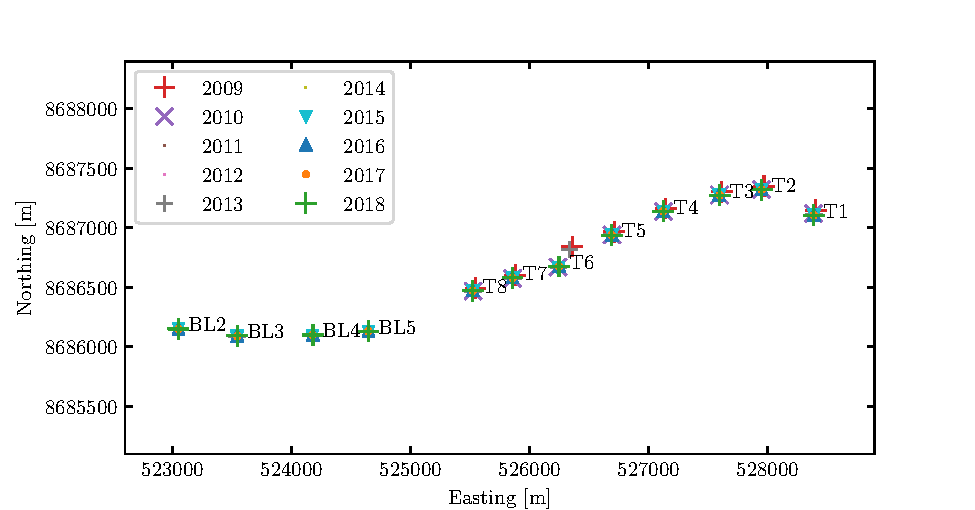
\includegraphics[width=\textwidth]{./figs/stakePositions.pdf}
    \caption{Positions of all stakes in the flow line on Blekumbreen and Tellbreen.
    The different markers distinguish the year of the measurement.}
    \label{GPS:fig:stakepos}
\end{figure}

Figure~\ref{GPS:fig:stakepos} shows the positions of the currently 12 different stake locations
on Blekumbreen and Tellbreen.
At those locations, a total of 26 measurements has been performed in 2018.
Additionally, all available data of stake positions since 2009 is shown on the figure.

The stakes spread over about 5 kilometers in east-west direction and 1.5 kilometers in north-south direction.
The coarse resolution of the figure shows a rough accordance of this years positions with last years values.

Figure~\ref{GPS:fig:T1_2d} shows all available data for T1 in a higher resolution.
The measurement of the position of T1-2017 (green) has been performed two times in order to estimate the uncertainty
of the method.
The two positions differ by 19\,cm and agree with each other within their uncertainties.



\begin{figure}[H]
    \centering
    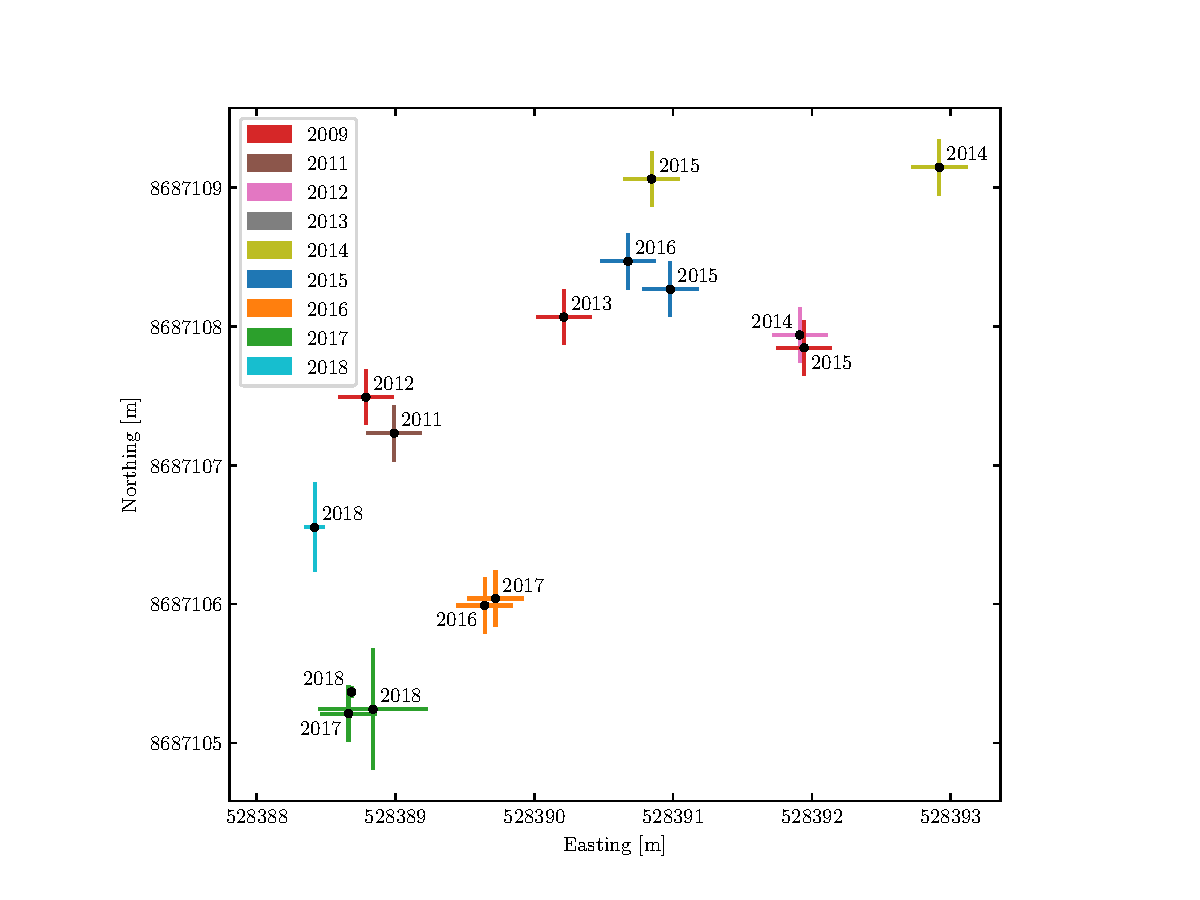
\includegraphics[width=\textwidth]{./figs/T1_2d.pdf}
    \caption{Measured positions at the location of stake T1 from 2011 to 2018.
    Different colors denote different stakes,
  	the year next to the stake positions is the year of the measurement.
    	At this location, a movement in south-east direction would be expected.
    	This is not identifiable using the data at hand.
 	Similar plots of the other 11 stake locations are situated in the appendix.}
    \label{GPS:fig:T1_2d}
\end{figure}


\begin{table}[h]
	\caption{Velocities of the stakes measured in 2018, calculated with equations~\ref{GPS:eq:v} and \ref{GPS:eq:sv}.
	All velocities have been calculated using last years position.
	If available, positions from 2016 and 2015 have also been used.
	To be able to assess the uncertainty of the velocities, some measurements have been performed twice.
	This is denoted by the suffices -i and -ii.}
	\centering
	%\scriptsize
	\begin{tabular}{lcccccc}
\toprule
  Stake name & Velocity (2017) [m/a] & Velocity (2016) [m/a] & Velocity (2015) [m/a] \\
\midrule
    BL2-2016 &       0.26 $\pm$ 0.21 &       0.21 $\pm$ 0.20 &                     - \\
    BL3-2016 &       0.16 $\pm$ 0.20 &       0.21 $\pm$ 0.18 &                     - \\
  BL4-i-2016 &       0.07 $\pm$ 0.26 &       0.08 $\pm$ 0.25 &                     - \\
 BL4-ii-2016 &       0.11 $\pm$ 0.56 &       0.05 $\pm$ 0.48 &                     - \\
  BL5-i-2017 &       1.75 $\pm$ 0.18 &                     - &                     - \\
 BL5-ii-2017 &       1.74 $\pm$ 0.24 &                     - &                     - \\
   T1-i-2017 &       0.09 $\pm$ 0.11 &                     - &                     - \\
  T1-ii-2017 &       0.19 $\pm$ 0.43 &                     - &                     - \\
     T2-2016 &       0.60 $\pm$ 0.24 &       0.28 $\pm$ 0.20 &                     - \\
   T2-i-2017 &       0.23 $\pm$ 0.30 &                     - &                     - \\
  T2-ii-2017 &       0.53 $\pm$ 0.51 &                     - &                     - \\
     T3-2017 &       0.10 $\pm$ 0.12 &                     - &                     - \\
     T4-2016 &       0.13 $\pm$ 0.38 &       0.17 $\pm$ 0.37 &                     - \\
     T5-2016 &       0.30 $\pm$ 0.33 &       0.12 $\pm$ 0.22 &                     - \\
     T6-2016 &       0.79 $\pm$ 0.31 &       0.12 $\pm$ 0.19 &                     - \\
     T7-2015 &       0.26 $\pm$ 0.27 &       0.10 $\pm$ 0.15 &       0.08 $\pm$ 0.19 \\
     T7-2017 &       1.33 $\pm$ 0.16 &                     - &                     - \\
     T8-2017 &       0.20 $\pm$ 0.24 &                     - &                     - \\
\bottomrule
\end{tabular}

	\label{GPS:tab:os_tab}
\end{table}

\begin{equation}
\label{GPS:eq:v}
v_\text{year} = \frac{\sqrt{(N_{2018}-N_{\text{year}})^2+(E_{2018} - E_{\text{year}})^2}}{t}
\end{equation}

\begin{equation}
\label{GPS:eq:sv}
\delta_{v_{\text{year}}} = \sqrt{\frac{
(\delta_{N_{2018}}^2 + \delta_{N_{\text{year}}}^2) * (N_{2018}-N_{\text{year}})^2 +
(\delta_{E_{2018}}^2 + \delta_{E_{\text{year}}}^2) * (E_{2018}-E_{\text{year}})^2}
{(N_{2018} - N_{\text{year}})^2+ (E_{2018} - E_{\text{year}})^2}}
\end{equation}




\subsection{Vertical velocity (mass balance)}